\documentclass[11pt]{article}
\usepackage[a4paper, total={7in, 10.5in}]{geometry}
\usepackage{graphicx}
\usepackage{float}
\usepackage{amsmath}
\usepackage{amssymb}
\usepackage{microtype}
\usepackage[font=small,labelfont=bf]{caption}
\usepackage[hidelinks]{hyperref}

\setlength{\parskip}{0.35em}
\setlength{\parindent}{0pt}

\title{Mid-Term Progress Report:\\[2pt]
Toward a Multi-Modal Foundation Model for LArTPC Reconstruction\\[4pt]
\large Data Generation, Detector Response, and a Compressible Signal Representation}
\author{Omar Alterkait}
\date{}

\begin{document}
\maketitle

\section{Summary of Progress}
The overarching goal of this project, as laid out in the proposal, is a multi-modal
Foundation Model (FM) that learns directly from the lowest-level detector signals of a
Liquid Argon Time Projection Chamber (LArTPC), namely the Time Projection Chamber (TPC) wire
planes and the Photon Detection System (PDS), in order to implicitly capture the detector
response and improve reconstruction. This mid-term report documents the progress made on
the two foundations that any such model requires before training can begin: \textbf{(i)} a
large-scale, high-fidelity, multi-modal simulation dataset, and \textbf{(ii)} a
principled front-end that turns the raw, noise-dominated waveforms into a compact,
denoised representation the model can actually ingest.

The central technical finding of this period is that the raw waveform stream is neither
directly trainable nor cheap to store: it is dominated by correlated (``coherent'') and
intrinsic electronics noise, and its native dimensionality (millions of samples per event
across both modalities) is prohibitive for a transformer. We show that a
\emph{wavelet-coefficient} representation, built from a coherent-noise remover followed by
a noise-relative wavelet sparsification, removes the noise almost to its statistical floor
while compressing each plane and each optical channel by one to two orders of magnitude, and
that the surviving coefficients are sparse and concentrated at physically meaningful scales.
This is precisely the property that makes an end-to-end Foundation Model on raw LArTPC data
computationally feasible. All of the analysis reported here has been implemented in a
dedicated, multi-backend signal-processing toolkit (\texttt{HELIX}) developed during this
period.

\section{A Scalable, Multi-Level Simulation Dataset}
A Foundation Model is only as good as the data it is pre-trained on. In collaboration with
the neutrino group at SLAC we have produced \textbf{Doraemon}, a large-scale simulated
dataset for a generic SBND-like LArTPC, now at the scale of \textbf{one million simulated
events}. The two modalities are generated from the \emph{same} underlying truth
interaction, so charge and light are \textbf{physically paired} event-by-event. This is a
property that is essential for the cross-modal self-supervised objectives (cross-view
completion, cross-modal masked auto-encoding) at the heart of the proposed model, and one
that would be impossible to obtain from real data.

\paragraph{Scalability.} The dataset is made possible by a GPU-resident simulation
(\texttt{JAXTPC}) that produces a full detector realization in \textbf{$\sim$1~second per
event on a single GPU}. This throughput is what turns a million-event, multi-modal corpus
from an aspiration into a routine production run, and it is what will allow the dataset to
continue to grow and to be regenerated as the detector model is refined.

\paragraph{The data hierarchy (``levels'').} Doraemon is stored and used at every level of
the physics chain, so that the Foundation Model can be trained on the rawest possible input
while still being evaluated and supervised against ground truth:
\begin{enumerate}\setlength{\itemsep}{2pt}
    \item \textbf{Truth:} per-interaction energy deposits, particle identities and
    positions on the charge side, and per-PMT photo-electron counts on the light side. This
    is the noise-free target and the label source for downstream probes.
    \item \textbf{Detector signals:} the charge drifted onto the wire planes and the
    scintillation light incident on the PDS, after the detector response is applied but
    before digitization.
    \item \textbf{Digitized raw waveforms:} the pedestal-subtracted ADC stream the model
    will actually see. This comprises three TPC wire planes (two induction planes, $U/V$, of
    1969 wires each with a bipolar response, and one collection plane, $Y$, of 1443 wires
    with a unipolar response) and 162 PDS channels (81 per side, east/west) with a realistic
    single-photo-electron response kernel.
    \item \textbf{Denoised wavelet-coefficient representation:} the compact, sparse
    substrate derived in this work (Sections~\ref{sec:coh} and~\ref{sec:opt}), which is the
    representation on which the Foundation Model is designed to operate.
\end{enumerate}
Because the truth level is retained alongside the raw level, every claim about denoising
fidelity below is measured against the exact noise-free signal, not against an approximate
reference.

\section{High-Fidelity Detector Response and Noise}
The value of pre-training on raw waveforms hinges on the raw waveforms being
\emph{realistic}: the model can only learn detector effects that the simulation actually
contains. During this period the simulation was upgraded from an idealized model to a
high-fidelity one whose \textbf{noise model is tuned to match MicroBooNE}, the most
thoroughly characterized SBN detector. Two noise components are applied on top of the clean
detector signals:
\begin{itemize}\setlength{\itemsep}{2pt}
    \item \textbf{Intrinsic noise:} per-wire independent, frequency-shaped electronics
    noise (equivalent-noise-charge tuned per plane), at the few-ADC level.
    \item \textbf{Coherent noise:} a correlated common-mode shared across each group of
    neighboring wires (a 64-wire readout block), with anti-correlation between adjacent
    blocks and a low-frequency ($1/f$-like) spectrum. Coherent noise is the dominant and
    most pernicious component: it is large ($\sim$2.5~ADC RMS common-mode) and, critically,
    it lives at the \emph{same coarse time scales where the physics signal lives}, so it
    cannot be removed by a naive frequency cut without damaging the signal.
\end{itemize}
We have verified on the optical channels that the injected noise is white and Gaussian at the
configured level with negligible ADC bias. This is exactly the regime in which real LArTPC
signal processing is hard, and it is the reason a dedicated denoising front-end, rather than
feeding raw ADC to the network, is required.

\section{The Denoising and Compression Problem}
Two obstacles stand between the raw Doraemon waveforms and a trainable Foundation Model
input. First, \textbf{noise}: as above, correlated noise overlaps the signal in scale and
must be removed in a signal-preserving way. Second, \textbf{dimensionality}: a single event
is a dense $\mathcal{O}(1969\times4321)$ image per induction plane plus $\sim$162 optical
waveforms of tens of thousands of samples each, i.e.\ millions of numbers, the overwhelming
majority of which are noise. A transformer whose cost is quadratic in token count cannot
consume this directly. Both obstacles are addressed by the same move: a
\textbf{wavelet decomposition} of each waveform, in which (a) coherent structure can be
identified and subtracted scale-by-scale, and (b) noise is thresholded away, leaving a
\emph{sparse} set of surviving coefficients that both denoises and compresses.

Our thresholding strategy throughout is \textbf{noise-relative VisuShrink} (a hard threshold
at $t=\kappa\,\sigma\sqrt{2\ln N}$ with a per-signal noise estimate $\sigma$). We validated
in a 100-event campaign that this is the correct criterion for a denoise-then-compress task:
content-relative alternatives (fixed energy or top-$k$ fractions) either leak on noise-only
regions or are blind to the noise level, whereas VisuShrink removes noise everywhere and
keeps signal in proportion to how far it stands above the noise. The single knob $\kappa$
sets the operating point on the rate-distortion curve.

\section{Coherent Noise and Decomposition on the TPC Wire Planes}
\label{sec:coh}
On the wire planes the pipeline is: \emph{coherent-noise removal} followed by
\emph{wavelet sparsification}. The coherent common mode is identical across the wires of a
readout block (a rank-1 component) and concentrates in the coarse wavelet bands, exactly
where the physics signal also sits, so it cannot be separated by a frequency cut. The removal
instead gates, scale by scale, on the contrast between the small, dense coherent common mode
and the large, sparse signal, subtracting the former while leaving the latter untouched.

Figure~\ref{fig:tpc_planes} shows the full pipeline on a collection-plane ($Y$) and an
induction-plane ($U$) event. Coherent removal erases the vertical common-mode striping; the
wavelet reconstruction then suppresses the residual incoherent noise, taking the noise RMS
from $\sim$3.2~ADC down to $\sim$0.3~ADC (a $\sim$10$\times$ reduction) while preserving the
tracks. The charge fidelity is $F_0=0.96$ on collection and $F_0=0.91$ on the harder bipolar
induction plane, at a per-plane \textbf{compression of $\sim$170--190$\times$}.

\begin{figure}[H]
    \centering
    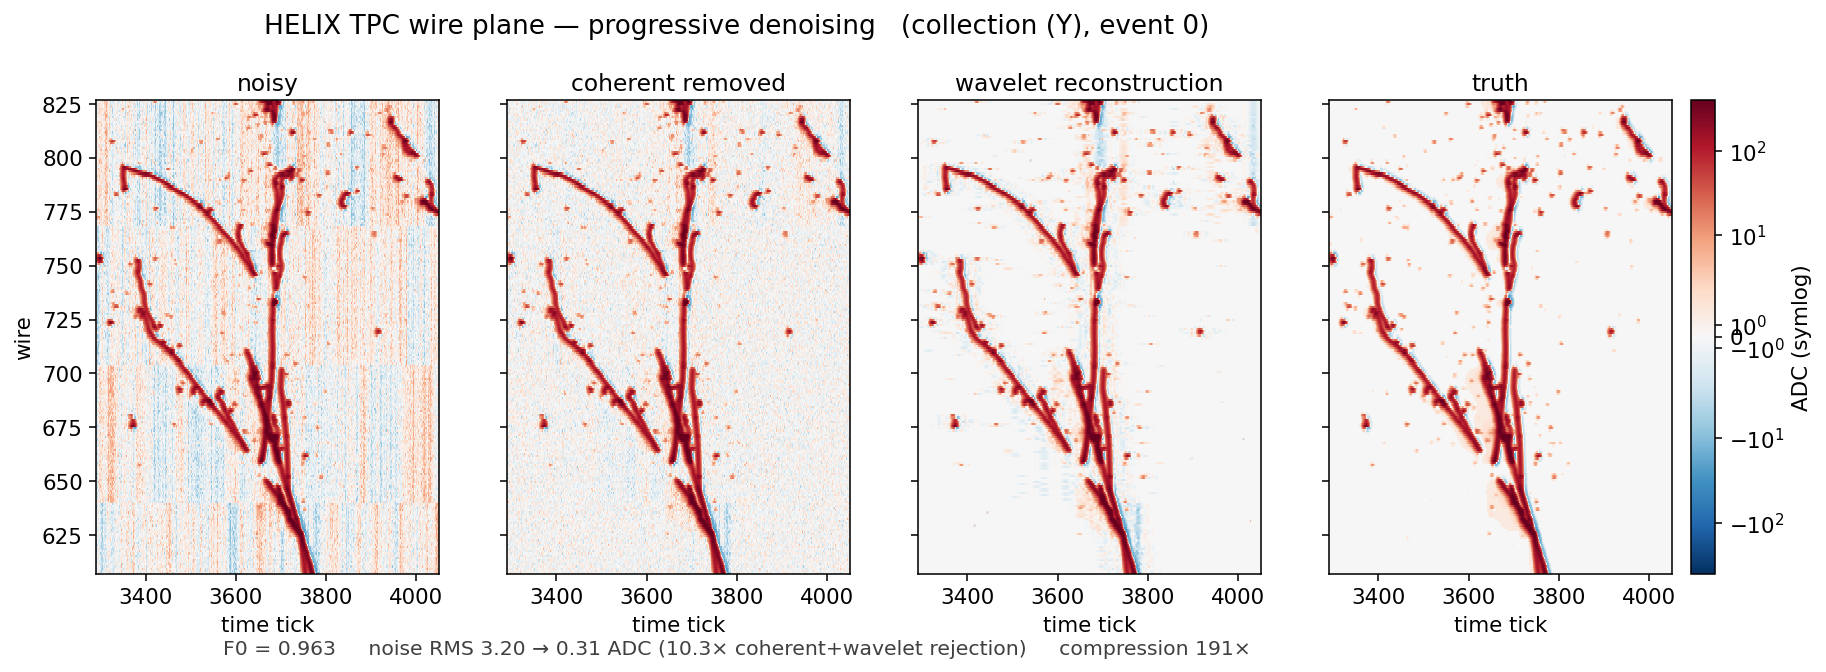
\includegraphics[width=\linewidth]{figures/tpc_denoise_Y.png}\\[4pt]
    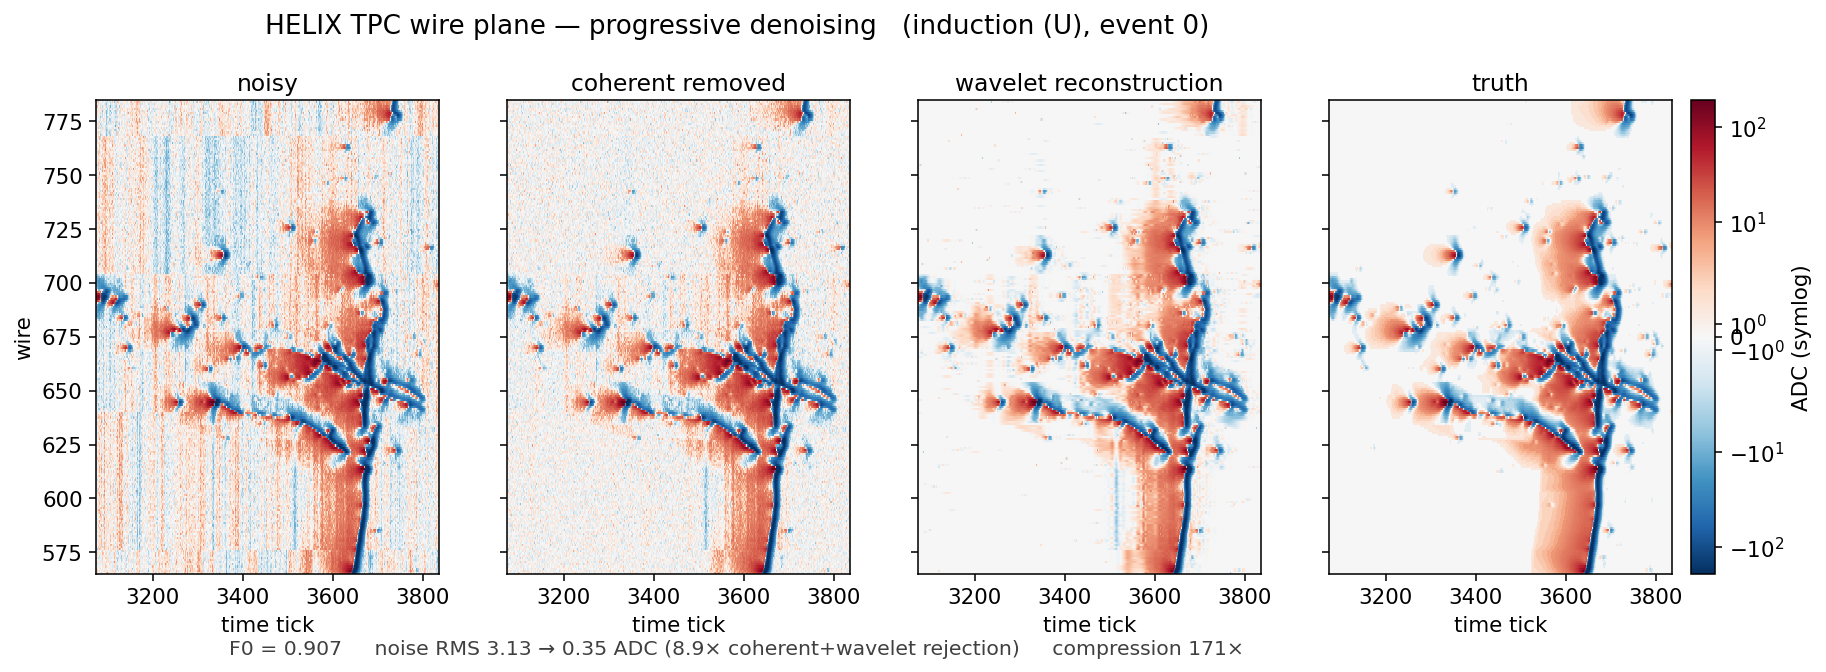
\includegraphics[width=\linewidth]{figures/tpc_denoise_U.png}
    \caption{Progressive denoising of the TPC wire planes in \texttt{HELIX}, shown for the
    collection plane ($Y$, top) and an induction plane ($U$, bottom): raw noisy image, after
    coherent-noise removal, after wavelet reconstruction, and the noise-free truth. Coherent
    removal eliminates the correlated vertical striping; wavelet sparsification suppresses
    the residual noise (RMS $3.2\!\rightarrow\!0.3$~ADC) while preserving the tracks, at
    $\sim$190$\times$ ($Y$, $F_0=0.96$) and $\sim$170$\times$ ($U$, $F_0=0.91$) compression.}
    \label{fig:tpc_planes}
\end{figure}

\paragraph{The representation scales with signal content, not raw size.} Running the full
pipeline at its default operating point over many events, each with a different amount of
true signal, Figure~\ref{fig:tpc_truepoints} plots the number of kept wavelet coefficients
against the number of true signal points per plane. The two grow together, at roughly $0.2$
kept coefficients per true signal point. Two comparisons matter here. Measured against the
true signal alone, the strictest baseline since it counts only the pixels that carry real
charge, the representation is already a few times smaller (the kept count sits well below the
diagonal). Measured against the full raw plane, an $\mathcal{O}(10^7)$-pixel image that is
overwhelmingly noise, it is far more compact still: the $\sim$170--190$\times$ compression of
Figure~\ref{fig:tpc_planes}. Either way its size is set by the physics content of the event,
not its raw dimensions, which is exactly the behaviour a token-based model needs.

\begin{figure}[H]
    \centering
    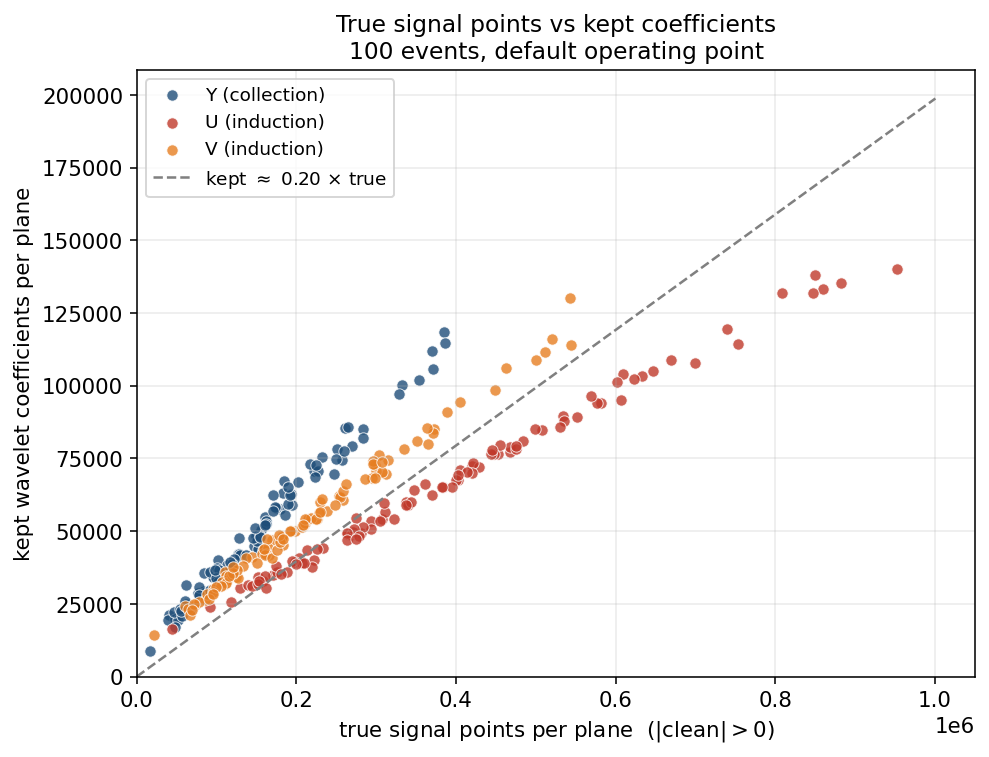
\includegraphics[width=0.72\linewidth]{figures/tpc_truepoints_vs_coeffs.png}
    \caption{Kept wavelet coefficients versus true signal points per plane, over 100 events
    at the default operating point (coherent removal plus VisuShrink-hard). Each marker is one
    plane of one event; the number of true signal points varies from event to event. The kept
    budget grows linearly with, and stays a few times below, the true signal size (dashed:
    kept $\approx0.2\times$ true); relative to the full raw plane it is more compact still, by
    the $\sim$170--190$\times$ of Figure~\ref{fig:tpc_planes}.}
    \label{fig:tpc_truepoints}
\end{figure}

\paragraph{Reconstruction accuracy inside and outside the signal.}
Figure~\ref{fig:tpc_within_outside} shows the reconstruction residual (recon $-$ true charge)
inside and outside the true signal, per plane. Inside the signal the residual is
$\sim$2.2--2.4~ADC RMS, the charge-reconstruction error on the tracks. Outside the signal the
true charge is exactly zero, so the residual is simply the reconstruction compared to zero: it
collapses to a sharp peak at zero ($\sim$0.35~ADC RMS), i.e.\ away from tracks the
reconstruction is essentially empty and hit-finding sees a clean field.

\begin{figure}[H]
    \centering
    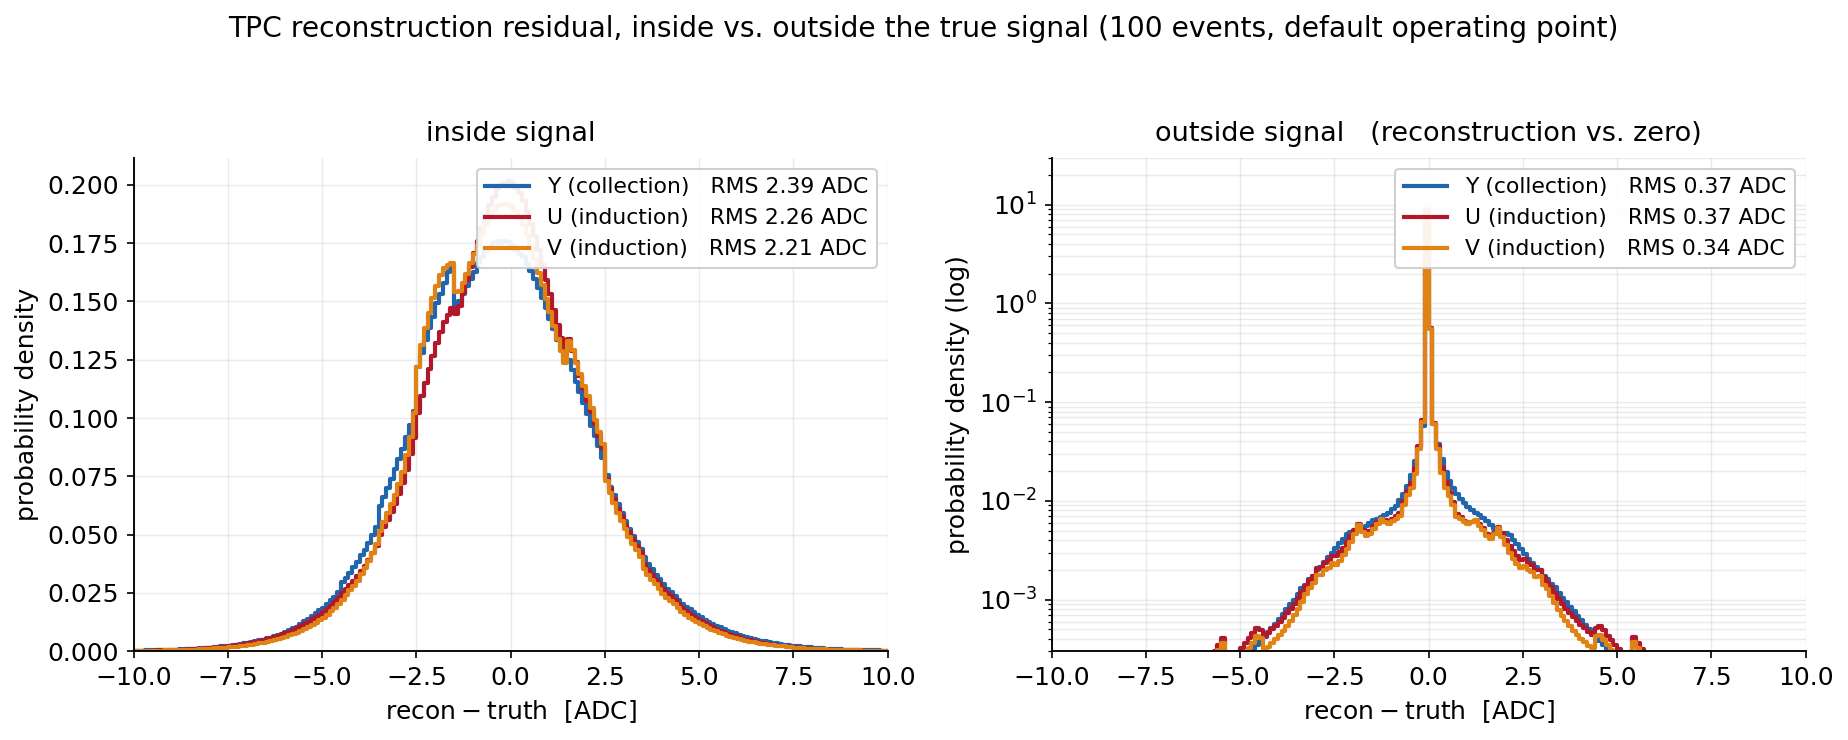
\includegraphics[width=\linewidth]{figures/tpc_resid_within_outside.png}
    \caption{Reconstruction residual (recon $-$ true charge) over 100 events at the default
    operating point, per plane. Left, inside the true signal: a broad distribution at
    $\sim$2.2--2.4~ADC RMS, the charge-reconstruction error on the tracks (the integer-ADC
    residual is dithered by its 1-ADC quantization for display). Right, outside the true
    signal: the true charge is zero there, so the residual is the reconstruction compared to
    zero. On a logarithmic density axis it is a sharp peak at zero (most off-signal pixels
    reconstruct to exactly zero) with rapidly falling tails, $\sim$0.35~ADC RMS.}
    \label{fig:tpc_within_outside}
\end{figure}

\section{Decomposition and Compression on the Optical (PDS) Waveforms}
\label{sec:opt}
The PDS waveforms are single-sided, large negative-going scintillation pulses on a white
$\sim$2.6~ADC noise floor. Figure~\ref{fig:opt_decomp} shows the multi-scale wavelet
decomposition of one PMT pulse: the pulse energy spreads coherently across a range of
scales, while the finest detail band ($D1$) is pure noise. This structure is what the
sparsifier exploits, discarding the noise-dominated fine scales and keeping the sparse set
of coefficients that reconstruct the pulse.

\begin{figure}[H]
    \centering
    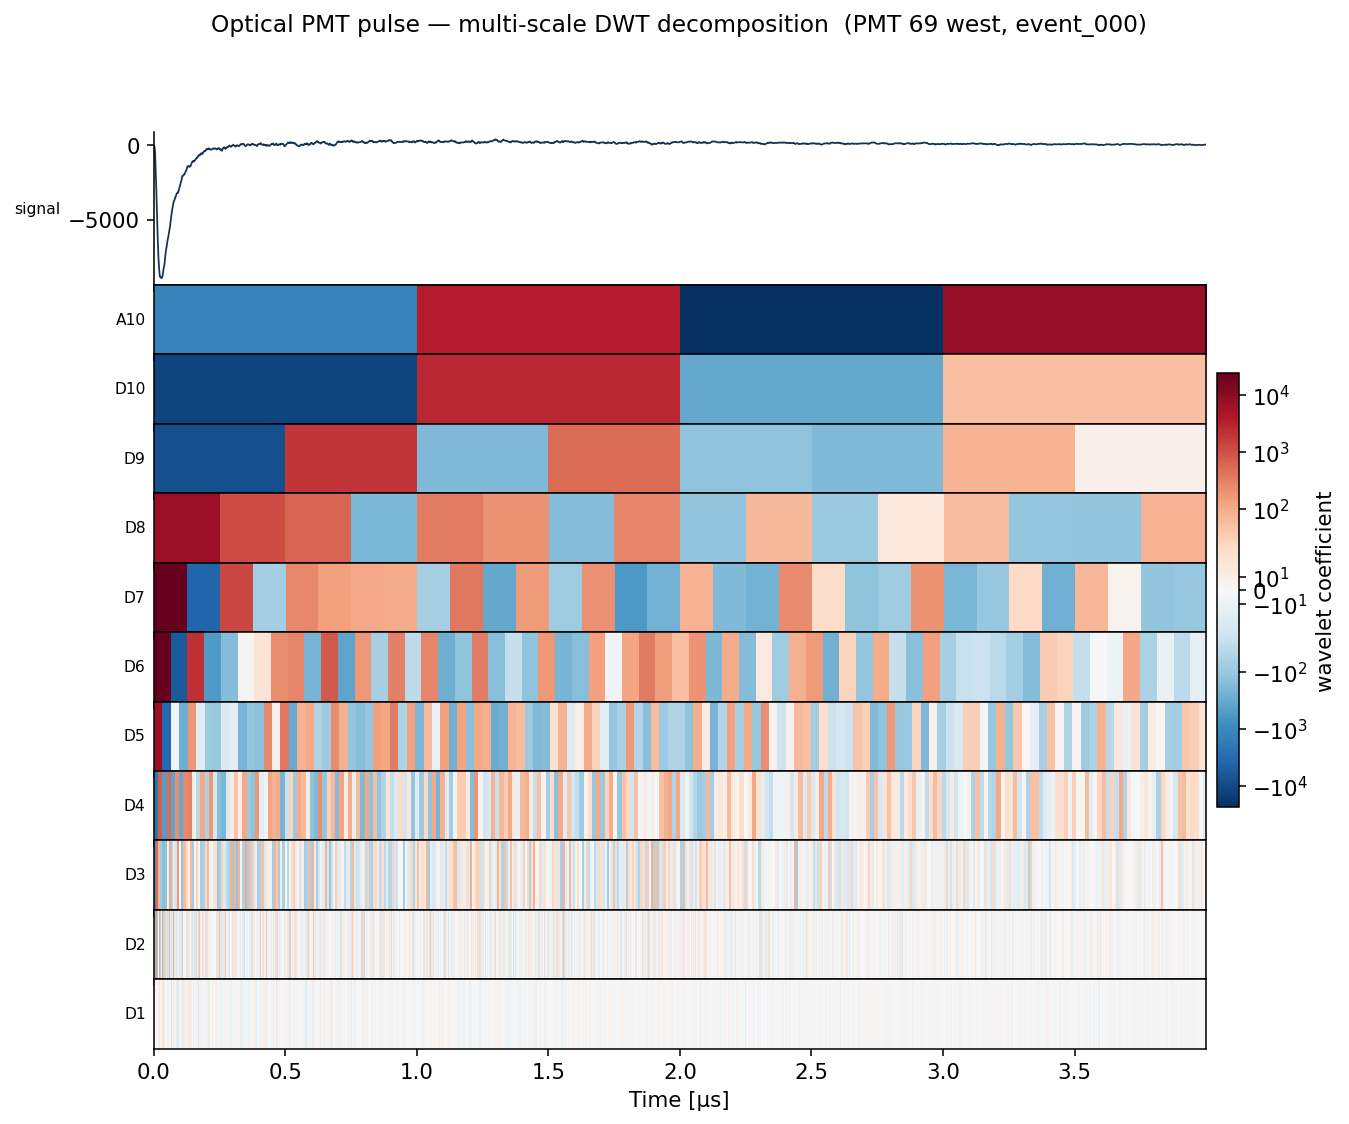
\includegraphics[width=0.78\linewidth]{figures/optical_decomposition.png}
    \caption{Multi-scale discrete wavelet decomposition (coif3, 10 levels) of a single PDS
    photo-multiplier pulse. The pulse projects coherently onto the coarse and mid-scale
    detail bands; the finest band ($D1$) is noise-dominated and is thresholded away.}
    \label{fig:opt_decomp}
\end{figure}

On average only $\sim$994 coefficients survive per signal chunk, out of tens of thousands,
concentrated at mid-scales; the survival fraction falls monotonically from the coarsest band
to essentially zero in the finest, noise-dominated band. The raw optical stream therefore
collapses to a small, structured set of tokens rather than a flat sea of samples, and its
size is set by the physics content of a chunk rather than its raw length.

Because the compression is achieved by \emph{denoising}, the natural axis on which to report
it is the reconstruction distortion relative to the noise floor.
Figure~\ref{fig:opt_rd} shows this rate-distortion frontier. At the \textbf{1$\times$
noise-floor operating point} the reconstruction RMS over the signal equals the intrinsic
noise ($\sim$2.6~ADC) at \textbf{$\sim$32$\times$ compression}; accepting $2\times$ or
$3\times$ the noise floor buys $\sim$50$\times$ or $\sim$82$\times$. In other words, all the
information below the noise floor is removed essentially for free, and the operating point is
a single, physically meaningful choice rather than an arbitrary rate target.

\begin{figure}[H]
    \centering
    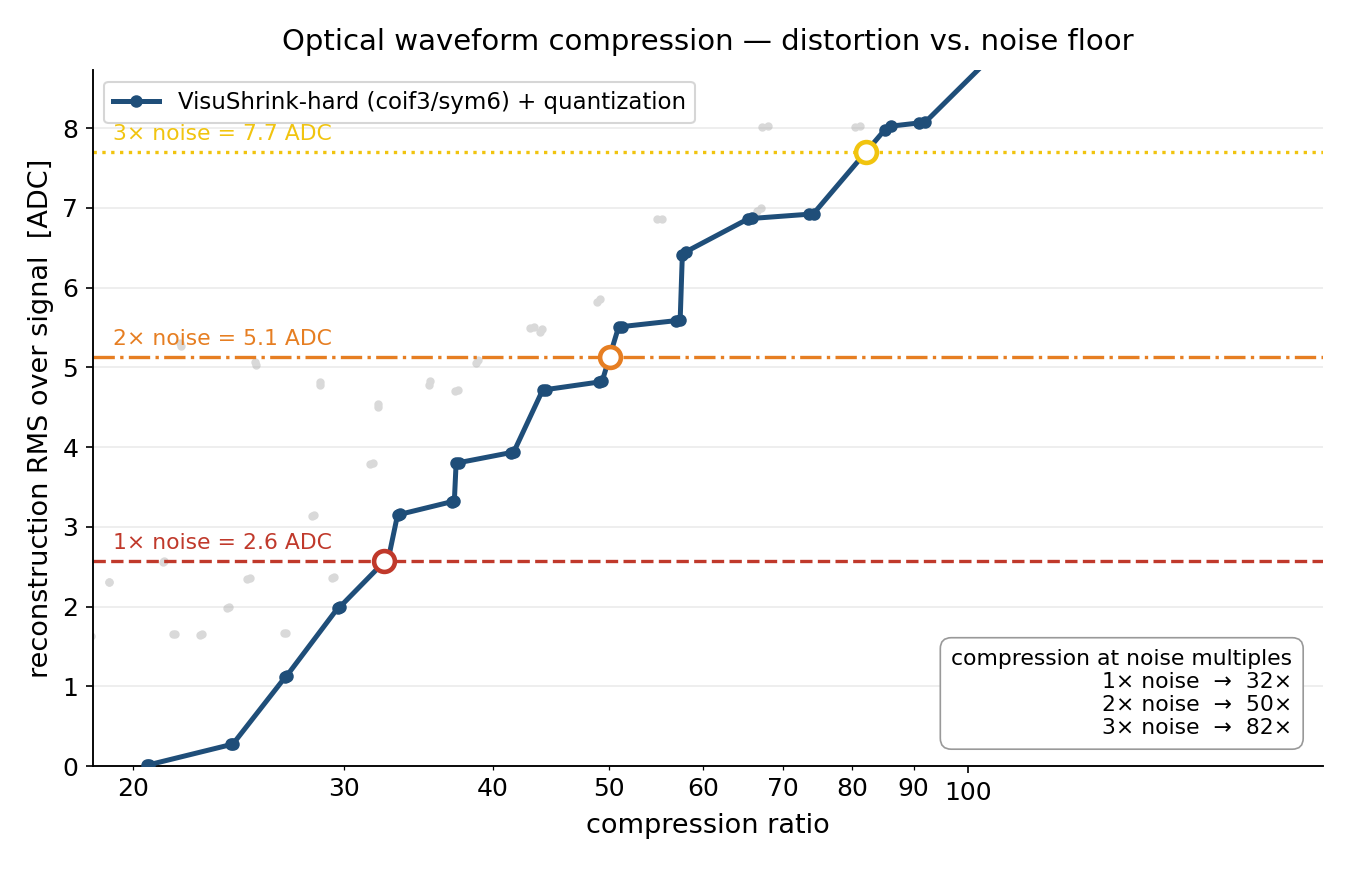
\includegraphics[width=0.82\linewidth]{figures/optical_rate_distortion.png}
    \caption{Optical rate-distortion frontier: reconstruction RMS over the signal versus
    compression ratio (VisuShrink-hard plus quantization). Horizontal lines mark
    1/2/3$\times$ the intrinsic noise floor; the corresponding compression ratios are
    32/50/82$\times$. The 1$\times$ point is the default operating point, denoising to the
    noise floor.}
    \label{fig:opt_rd}
\end{figure}

Figure~\ref{fig:opt_event} shows the result on a full 85-PMT event side: the whole-event
display is visibly denoised at $\sim$33$\times$, with the prompt scintillation flash preserved.

\begin{figure}[H]
    \centering
    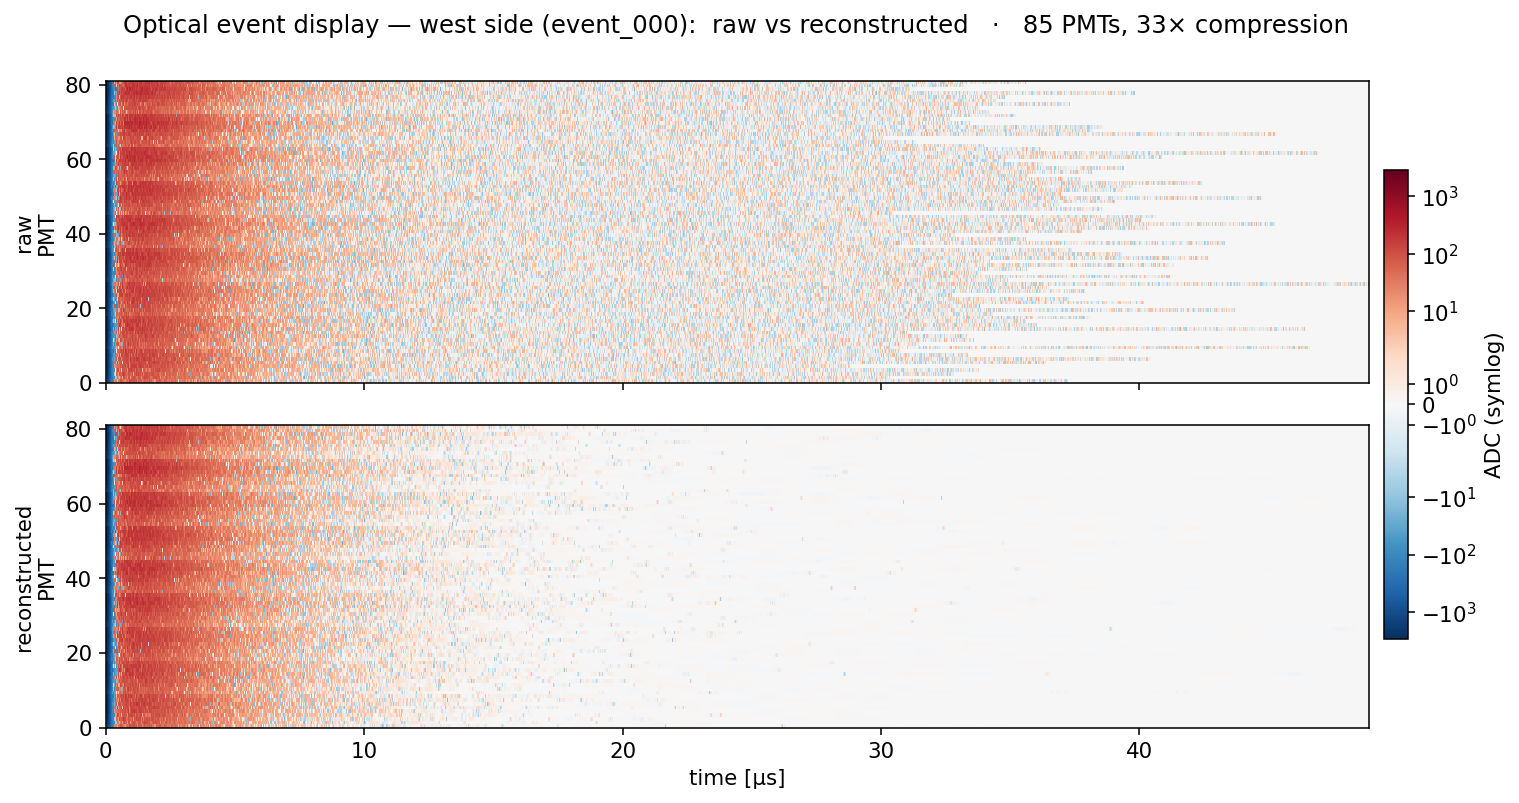
\includegraphics[width=\linewidth]{figures/optical_event_2d.png}
    \caption{Full optical event display (one side, 85 PMTs): raw (top) versus reconstructed
    (bottom). The prompt scintillation flash is preserved while the noise tail is removed,
    at $\sim$33$\times$ compression.}
    \label{fig:opt_event}
\end{figure}

\section{Feasibility for the Foundation Model}
Taken together, the results above establish that raw LArTPC waveforms can be turned into a
representation that a Foundation Model can consume:
\begin{itemize}\setlength{\itemsep}{2pt}
    \item \textbf{The noise is removed to its statistical floor} on both modalities, in a
    signal-preserving way (charge fidelity $F_0 \gtrsim 0.9$ on the wire planes and
    reconstruction to the noise floor on the PDS). The model is therefore trained on the
    physics content, not on the electronics noise, and, because the truth level is retained,
    the denoised target is exact.
    \item \textbf{The dimensionality collapses by one to two orders of magnitude}
    ($\sim$170--190$\times$ per TPC plane and $\sim$32$\times$ per optical channel at the
    noise floor), bringing the per-event token count into a range a transformer can handle
    while keeping quadratic-attention cost tractable.
    \item \textbf{The surviving coefficients are sparse and structured}, concentrated at a
    handful of physically meaningful scales, with a monotone coarse-to-fine survival
    profile. This is a natural, compact tokenization: a small set of (scale, position,
    value) elements per plane and per channel, shared in form across both modalities and
    across the continuous time-scale axis that links them.
    \item \textbf{The representation is paired and multi-modal by construction}: charge and
    light are derived from the same truth and share a common time-scale description, which
    is what the proposed cross-modal self-supervised objectives require.
\end{itemize}

\section{Status Against the Aims and Next Steps}
This period delivered the data and representation infrastructure that Aims~1 and~2 depend
on: a scalable, high-fidelity, paired million-event dataset (Aim~2's pre-training corpus),
and a validated, compact, denoised coefficient representation of the raw waveforms that
makes a transformer over raw LArTPC data tractable (a prerequisite for the scalable
architecture of Aim~1). The full multi-backend \texttt{HELIX} toolkit implementing the
coherent-removal and sparsification pipeline for both modalities is complete and validated
on real Doraemon events.

The immediate next steps are to (i) finalize the coefficient-level dataloader that streams
the paired representation for both modalities, and (ii) begin self-supervised pre-training of
the multi-modal architecture on this substrate, followed by the downstream evaluation and
comparison against state-of-the-art reconstruction described in Aim~3. The compression and
denoising results reported here de-risk the central computational feasibility question and
put the project on track for the model-development phase.

\begin{thebibliography}{9}
\bibitem{SBNProgram} R.~Acciarri \emph{et al.} (MicroBooNE, LAr1-ND, and ICARUS-WA104
Collaborations), ``A Proposal for a Three Detector Short-Baseline Neutrino Oscillation
Program in the Fermilab Booster Neutrino Beam,'' arXiv:1503.01520 (2015).
\bibitem{uBNoise} R.~Acciarri \emph{et al.} (MicroBooNE Collaboration), ``Noise
Characterization and Filtering in the MicroBooNE Liquid Argon TPC,'' JINST \textbf{12},
P08003 (2017).
\bibitem{uBSigProc} C.~Adams \emph{et al.} (MicroBooNE Collaboration), ``Ionization electron
signal processing in single phase LArTPCs,'' JINST \textbf{13}, P07006/P07007 (2018).
\bibitem{VisuShrink} D.~L.~Donoho and I.~M.~Johnstone, ``Ideal spatial adaptation by wavelet
shrinkage,'' Biometrika \textbf{81}, 425 (1994).
\bibitem{MAE} K.~He \emph{et al.}, ``Masked Autoencoders Are Scalable Vision Learners,''
CVPR (2022).
\bibitem{SPINE} F.~Drielsma \emph{et al.}, ``Scalable Particle Imaging with Neural
Embeddings (SPINE),'' and the \texttt{lartpc\_mlreco3d} framework.
\bibitem{PolarMAE} S.~Young \emph{et al.}, ``PoLAr-MAE: Point-cloud Masked Autoencoders for
Liquid Argon TPC data,'' arXiv:2502.02558 (2025).
\end{thebibliography}

\end{document}
